%----------------------------------------------------------------------------
\chapter{Automatizált feladatkiértékelő modul}\label{chapter:exercise}
%----------------------------------------------------------------------------

A Jporta legfőbb alkotóeleme a feladatok leírásáért és a kiadott feladatokra érkezett megoldások automatizált kiértékeléséért felelős modul.
A portálnak ebben az újabb változatában fontos cél, hogy ez az alrendszer flexibilisebb legyen, mint az eddigi megoldások.
Ezt a flexibilitást egy általánosabb, de mégis egységes felépítés alkalmazásával igyekeztem elérni.
Az általam megtervezett rendszer a programnyelvek használatához kapcsolódó eszközök (pl. fordítók, interpreterek, tesztelési környezetek) alacsonyszintű működését egy közös, magasabb szintű absztrakció mögé rejti, melynek hatására a rendszer bővíthetősége megnő, és akár nem programozási jellegű feladatok készítésére is alkalmassá válik.

Ebben a fejezetben végigvezetem az olvasót a modul megtervezésének folyamatán, a követelmények összegyűjtésétől a megtervezett rendszer működésének és használatának leírásán át, egészen az implementációhoz szükséges technológiák bemutatásáig.

\section{Követelmények}\label{section:requirements}
A tervezés első lépése a tervezendő modullal szemben támasztott követelmények felmérése, amit a már meglévő munka elemzésével kezdtem.
A modul követelményeinek túlnyomú részét \cite{Ory13} már azonosította, miközben a portál egészére nézve végezte el ezt a feladatot.
A \cite{Kalman14} szakdolgozat tovább pontosította a követelményeket, miközben a portál más aspektusainak fejlesztésén dolgozott.
Az általuk feltárt követelmények a következők:
\begin{enumerate}
    \item A hallgató listázhatja és megtekintheti a számára kiosztott feladatokat.
    \item A hallgató a feladatokhoz megoldást adhat be.
    \item A hallgató megtekintheti korábban beadott megoldásait és azok eredményeit.
    \item Az oktató új feladatot hozhat létre.
    \item \label{req:specification} A feladatok tartalmaznak feladatkiírást, amely lehet statikus vagy dinamikusan generált.
    \item A feladatoknak része lehet egy vagy több fájl, amelyeket az oktató ad meg.
    \item A feladatoknak része lehet egy vagy több fájl, melyet a hallgatónak kell beadnia.
    \item A feladatok tartalmaznak automatikusan végrehajtható ellenőrzéseket.
    \item Az oktató feladatot adhat ki hallgatónak.
    \item Az oktató a feladatra beadott megoldásokat listázhatja, megtekintheti azok tartalmát, eredményét.
    \item A rendszer bővíthető új nyelvek, környezetek, eszközök támogatásával.
    \item Egy feladatkörben több alternatív eszköz (pl. GCC és Clang C fordítók) támogatása, akár egy feladaton belül is.
    \item \label{req:isolation} A megoldások kiértékelése izolált környezetben történik.
    \item \label{req:distributed} A kiértékelés elosztott rendszerben, tetszőleges számú gépen működik.
\end{enumerate}
Ezek a követelmények részben megegyeznek a Cporta eredeti követelményeivel, illetve tartalmaznak a Cporta használata közben megfogalmazott igényeket is.
A Jporta első, demó változatának próbája során azonban további igények fogalmazódtak meg a felhasználókban, melyek a feladatkiértékelő modult is érintették.
Ezek alapján én az alábbi kiegészítéseket teszem a követelmények már meglévő listájához:
\begin{enumerate}[resume]
    \item \label{req:manual} A feladatok tartalmazhatnak emberi beavatkozást igénylő ellenőrzéseket.
    \item \label{req:traceability} A kiértékelés folyamata legyen nyomonkövethető.
\end{enumerate}

A követelmények nagy része nem igényel magyarázatot, ám van néhány, amelyekről szeretnék még pár szót szólni.

Az \ref{req:specification}. követelmény a feladatkiírás szövegének dinamikus generálhatóságát írja elő.
Ez azt jelenti, hogy a feladatkiírás hallgatónként eltérő lehet, amely eltérés a hallgató személyétől, pontosabban a személyéhez kapcsolódó, rendelkezésre álló információktól függ.
Ilyen adat lehet például a hallgató neve, Neptun kódja, e-mail címe, felhasználóneve, stb.
Ezenkívül, a generáláshoz felhasználható bármilyen, a generálás pillanatában rendelkezésre álló erőforrás, pl. az oktató által megadott fájl, kerülendő azonban a nem megismételhető műveletekkel szerezhető adatok felhasználása (pl. aktuális idő lekérdezése, az operációs rendszer véletlenszám generátorának használata).

A \ref{req:isolation}. követelmény előírja, hogy a feladatok kiértékelése izolált környezetben történjen.
Ez nagyon fontos kitétel a rendszer biztonsága és stabilitása szempontjából.
Az izoláció egyrészt védi a gazda rendszert, amelyben a kiértékelések végbemennek, másrészt az egyidejűleg futó kiértékeléseket is védi egymástól.

A \ref{req:manual}. követelményre azért van szükség, mert a informatika jelenlegi eszközeivel nem minden ellenőrzés valósítható meg, néha elkerülhetetlen az emberi beavatkozás szükségessége.
A rendszer előző változataiban azonban nem volt ilyen jellegű funkció, a kiértékelés minden lépése automatizáltan történt.
Ez az új igény azonban jelentős változással jár a kiértékelés menetében, ugyanis egy potenciálisan végtelen, de mindenképp az eddigiekhez képest hosszú várakozást -- max. pár 100 milliszekundum kontra percek, órák, napok -- iktat be a folyamatba.
Ahhoz, hogy ezalatt a várakozás alatt a kiértékelést végző rendszer erőforrásai ne legyenek feleslegesen lefoglalva, a kiértékelés végrehajtása nem történhet egyetlen folytonos menetben, szükség van a folyamat állapotának elmentésére, majd visszatöltésére és a kiértékelés folytatására az emberi beavatkozás elvégzése után.

A \ref{req:traceability}. követelményre a rendszer auditálhatósága miatt van szükség, de a feladatokban, esetleg a feladatot kiértékelő rendszerben előforduló hibák feltárását és kezelését is megkönnyíti.
A követelmény teljesítéséhez rendelkezésünkre kell állnia a kiértékelés mindenkori állapotának, illetve a kiértékelés során keletkezett részeredményeknek.

\section{A feladatkiértékelő modul működése}\label{section:execution-procedure}
Az újratervezett feladatkiértékelő modul felépítését a \textit{csővezetékek és szűrők} (\textit{pipes and filters}, \cite{PipesAndFilters}) architektúrális tervezési mintára alapoztam.
A \textit{szűrők} a feladatok kiértékelési lépéseit (pl. fordítás, futtatás, tesztelés) reprezentálják, míg a \textit{csővezetékek} a lépések közötti adatáramlást.
A \ref{figure:example-pipeline}. ábrán a leggyakrabban előforduló feladat felépítés sematikus képe látható, melyen a különféle ``dobozok'' testesítik meg a szűrőket, a köztük vezető nyilak pedig a csővezetékeket, melyek egyúttal az adatáramlás irányát is szemléltetik.
Ahogy az ábrán is jól látható, a szűrőket három csoportra oszthatjuk: \textit{források}, \textit{átalakítók} és \textit{nyelők}.
Az ábrán látható paralelogrammák a források, a téglalapok az átalakítók, a hengerek pedig a nyelők.

\begin{figure}[h]
    \centering
    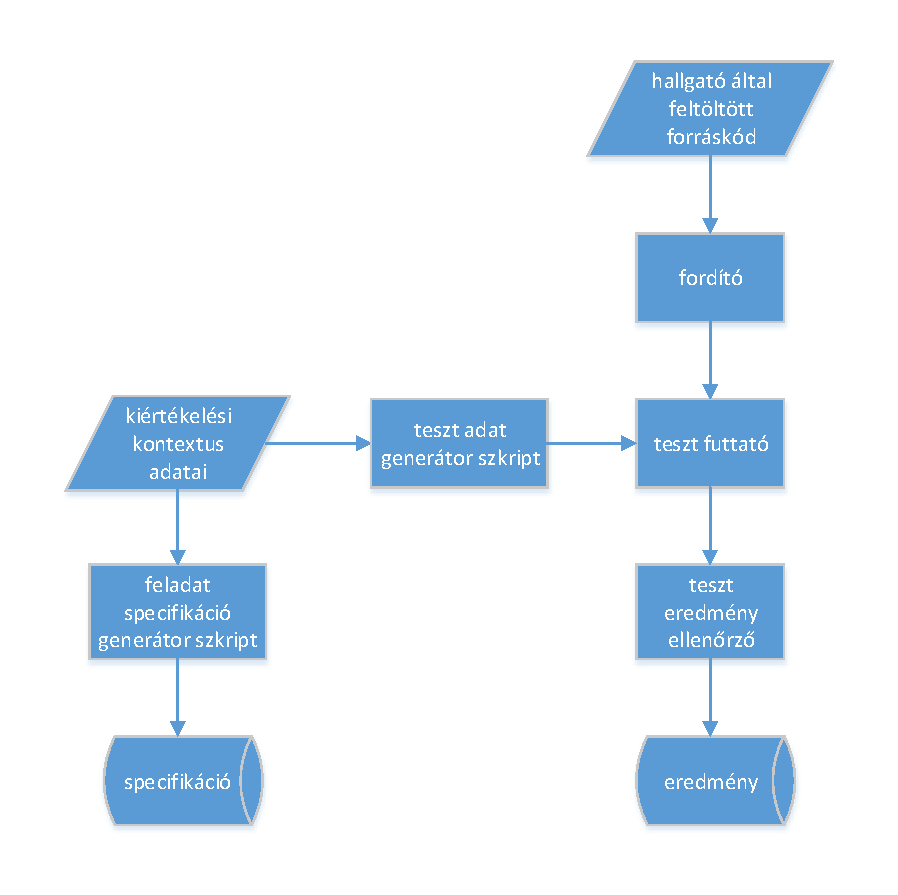
\includegraphics[width=0.95\textwidth]{figures/example-pipeline}
    \caption{A legjellemzőbb feladatstruktúra}
    \label{figure:example-pipeline}
\end{figure}

Az így felépített struktúra mindig egy irányított gráfot határoz meg, melynek csúcsai a szűrők, élei pedig a csővezetékek, az élek iránya pedig a szűrők közti adatáramlás iránya.
Ha ennek a gráfnak az éleit megfordítjuk, egy \textit{függőségi gráfot} kapunk, melynek segítségével meghatározhatjuk a kiértékelés lépéseinek sorrendjét.
Ahhoz, hogy a feladat kiértékelhető legyen, \textbf{a függőségi gráfnak körmentesnek kell lennie}. \cite{wiki:DependencyGraph}

A kiértékelés kezdetben mindig a függőségi gráf egy 0 bemeneti fokszámú csúcsából -- az eredeti gráfban nyelő -- indul.
A következő lépés, hogy meghatározzuk azon csúcsok halmazát, amelyektől a kiértékelendő csúcsunk közvetlenül függ.
Mielőtt ezt a csúcsot kiértékelhetnénk, az összes ebben a halmazban lévő csúcsnak ki kell lennie értékelve, ezért ezt az algoritmust a halmaz elemeire is rekurzívan alkalmazzuk.
Ha olyan csúcsot találunk, amelynek nincs függősége -- azaz, 0 a kimeneti fokszáma; az eredeti gráfban forrás --, akkor azt a csúcsot azonnal kiértékelhetjük.
Mivel a gráfról kikötöttük, hogy körmentesnek kell lennie, csúcsainak száma pedig véges, az algoritmusunk véges számú lépésben kiértékeli a feltárt részgráfot.
Ez az algoritmus soros végrehajtás esetén ideális.
A kiértékelés hatékonysága növelhető, ha a már kiértékelt csúcsok eredményeit egy gyorsítótárban eltároljuk, így ha több csúcs is függ ugyanattól az eredménytől, a kiértékelést akkor is csak egyszer végezzük el (lásd \cite{wiki:Memoization}).

Egy másik lehetséges algoritmus, ha a függőségi gráfot a lehető legkevesebb szintre osztjuk úgy, hogy az egy szinten lévő csúcsok között ne legyen függőség.
Az azonos szinten lévő csúcsok egymástól függetlenül kiértékelhetőek, amit kihasználhatunk, ha lehetőségünk van párhuzamos végrehajtásra.

A ``pipe'' és ``filter'' szavakat az informatikában sok esetben használják, gyakran hasonló, de eltérő jelentésekkel.
Ezzel összhangban a Python nyelvben a ``filter'' szó egy beépített függvényre hivatkozik, és a ``pipe'' szó is sok beépített függvénykönyvtárban előfordul.
A félreértések elkerülése végett a továbbiakban a szűrőket \textit{blokkoknak} (\textit{block}), a csővezetékeket pedig \textit{azonosítóknak} (\textit{handle}) fogom nevezni.
Ez azért is előnyös, mert a szóhasználat jobban utal a minta konkrét megvalósítására, amely jobban hasonlít a matematikai feladványokból ismert ``műveleti gépekhez''.

\section{Feladatok leírása}
Az előzőekben vázoltak alapján, szinte adja magát a feladatok leírására szolgáló modell, melynek két központi eleme a \texttt{Block} és a \texttt{Handle} osztályok.
A \texttt{Block} absztakt ősosztályként szolgál a különböző funkciókat (pl. fájlfeltöltés, fordítás, futtatás, ellenőrzés) megvalósító blokk osztályok számára.
Az ezekből példányosított blokkok pontosan egy feladatnak részei, melyet az \texttt{Exercise} osztály modellez.
A blokkokat a \texttt{Handle} osztály példányai kötik össze, melyek egy feladaton belül egyedi névvel rendelkeznek.
Ez az összeköttetés azonban nem közvetlen, hanem a \texttt{Provider} és a \texttt{Consumer} osztályok példányain keresztül történik.
Minden \texttt{Handle} példány pontosan egy \texttt{Provider} példányhoz tartozik, amelyek szintén pontosan egy blokkhoz tartoznak.
Ez a kapcsolat jelzi, hogy melyik blokk kiértékelése állítja elő az azonosító által megnevezett erőforrást, vagyis ezek a blokk kimenetei.
A \texttt{Consumer} osztály példányai ennek a kapcsolatnak a párját testesítik meg, vagyis hogy az erőforrást mely blokkok használják fel kiértékelésükkor, mik a blokk bemenetei.
Minden \texttt{Consumer} példány pontosan egy blokkhoz kapcsolódik, ám egy \texttt{Handle} példányhoz több \texttt{Consumer} is kapcsolódhat, hiszen ugyanazt az erőforrást több blokk is felhasználhatja.
Minden blokkra igaz, hogy nulla vagy több \texttt{Provider} és \texttt{Consumer} példányhoz kapcsolódik.
Az előző részekben említett \textit{források} azok a blokkok lesznek, amelyek nem kapcsolódnak \texttt{Consumer} példányhoz.
Hasonlóképp, a \texttt{Provider}-ektől mentes blokkok lesznek a \textit{nyelők}.
Az itt leírt modellosztályokat szemléltető UML osztálydiagram a \ref{figure:exercise-uml-cd}. ábrán látható.

\begin{figure}[h]
    \centering
    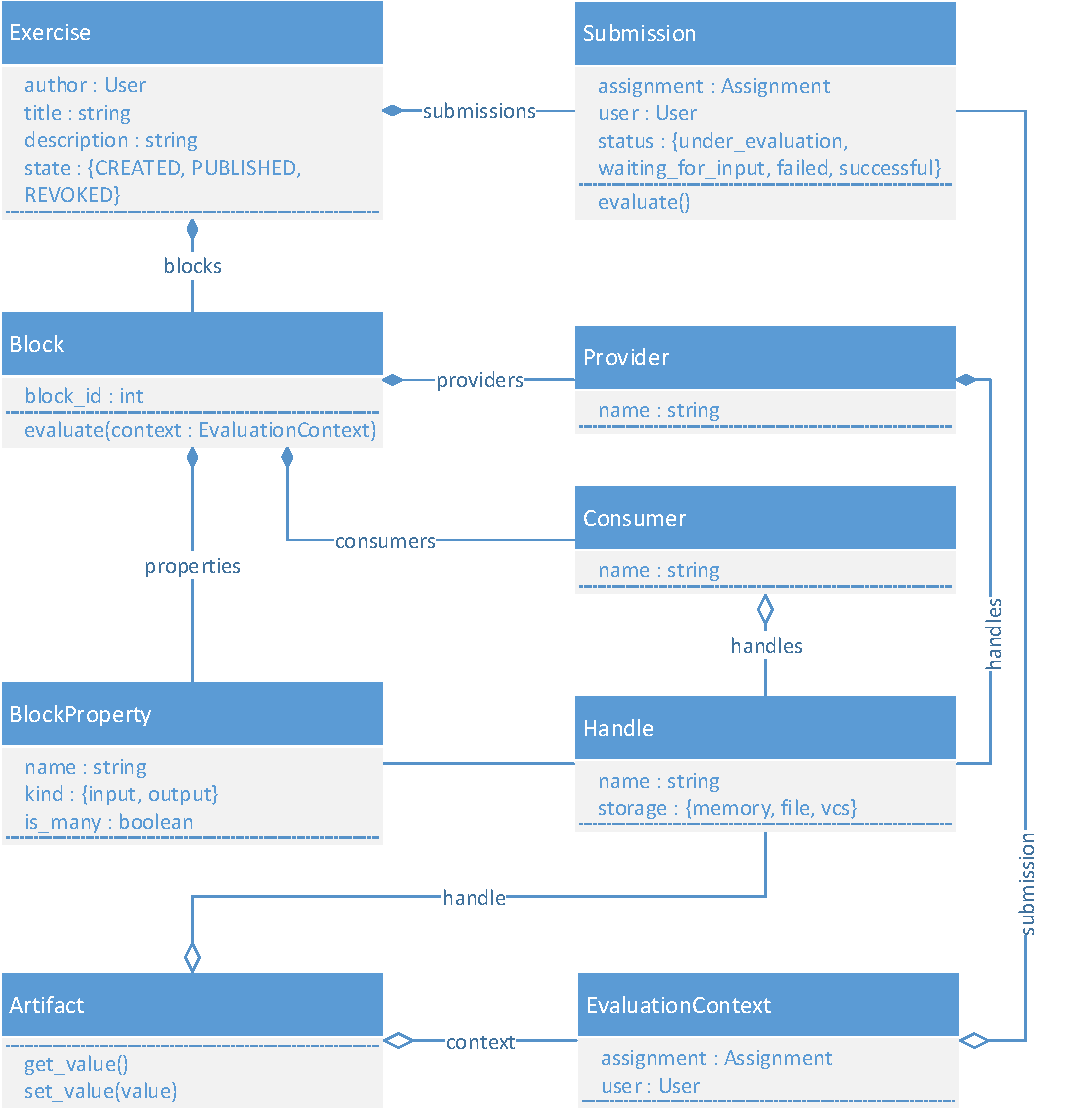
\includegraphics[width=\textwidth]{figures/exercise-uml-cd}
    \smallskip
    \caption{Feladatleíró modul UML osztálydiagramja}
    \label{figure:exercise-uml-cd}
\end{figure}

Mivel a \texttt{Block} osztály csak ősként szolgál a különböző blokktípusok számára, minden egyedi funkciót az ebből származtatott osztályokban kell megvalósítani.
A blokkok be- és kimeneteit a \texttt{Block\-Property} osztály példányai jelölik a Django modellek \texttt{Field}-jeihez hasonló, deklaratív megoldással.
Amikor a Python értelmező betölti a \texttt{Block} osztály egy leszármazottját, a típus létrehozásának folyamatába beavatkozik a \texttt{Block\-Metaclass} osztály, ami a Python \texttt{\_\_new\_\_} speciális metódusát definiálja felül, és a \texttt{Block} osztály meta\-class-aként van megjelölve. \cite{PythonMetaclass}
Ez a metódus a típus definiciójában található összes \texttt{Block\-Property} típusú attribútumot lecseréli egy \texttt{Block\-Property\-Descriptor} típusú attribútumra, aminek átadja az attribútum nevét és paramétereit, illetve a típus egy speciális attribútumába feljegyzi a tulajdonság nevét.
Ez utóbbi lista alapján tudja azonosítani a blokk osztály, hogy mely attribútumai be- és kimenetek.
A \texttt{Block\-Property\-Descriptor} példányok a Python nyelv \textit{leíró} (\textit{descriptor}) mintáját valósítják meg.
Ez az osztály ugyan felüldefiniálja a mintában található mindhárom speciális metódust (\texttt{\_\_get\_\_}, \texttt{\_\_set\_\_} és \texttt{\_\_delete\_\_}), azonban csak a \texttt{\_\_get\_\_} metódust valósítja meg.
Ez a következő speciális működést vonja magaután: amikor egy blokk osztály példányának be- vagy kimenetet reprezentáló attribútumát elérjük (értsd: \texttt{blokk\_peldany.attributum}), akkor ez a felüldefiniált \texttt{\_\_get\_\_} metódus hívódik meg úgy, hogy a leírót, a blokk példányt és a blokk típust (osztályt) kapja meg paraméterül. \cite{PythonDescriptors}
Ez a metódus a \texttt{Block\-Property\-Instance} osztály egy példányával tér vissza.
Ez az objektum az eredeti \texttt{Block\-Property} paraméterein és a hozzá vezető attribútum nevén kívül magára a tartalmazó blokk példányra is tartalmaz egy referenciát, amelyen keresztül manipulálni tudja azt.

A blokkok egyedi kiértékelési algoritmusát a leszármazott osztály \texttt{evaluate} metódusa valósítja meg.
Ez a metódus paraméterként megkapja a blokk referenciáját és a blokk kiértékelésének kontextusát (lásd \ref{section:submission-evaluation}. szakasz), és ezeket felhasználva elvégzi a kimeneti értékei kiszámításához szükséges számításokat, majd a kontextusban beállítja a kimeneteinek megfelelő értékeket.

\section{Feladatok készítése}\label{section:exercise-creation}
A rendszer, általános felépítése miatt, nem tartalmaz sok megkötést a leírható feladatokra: az egyszerű PDF formátumú beadandók feltöltésétől egészen a grafikus felülettel rendelkező, interaktív házi feladatokat fordító, futtató és tesztelő beadásokig szinte bármilyen feladat összeállítható benne.
Ahhoz, hogy ez a változó komplexitású munkafolyamat felhasználóbarát maradjon, egy egyszerű felületre van szükség, amely nagy összetettségű feladatok esetén sem válik kezelhetetlenné.

A hasonló felépítésű, adatfolyamokra alapozó modellek manipulációjára általában vizuális, csomópont alapú szerkesztőket szoktak alkalmazni.
Ezek az eszközök azért nagyon jól használhatóak, mivel a modell kézenfekvő reprezentációját használják a vizualizációhoz, amely nagyban segíti a megértést, és egy intuitív interfészt biztosít.
\begin{figure}[h]
    \centering
    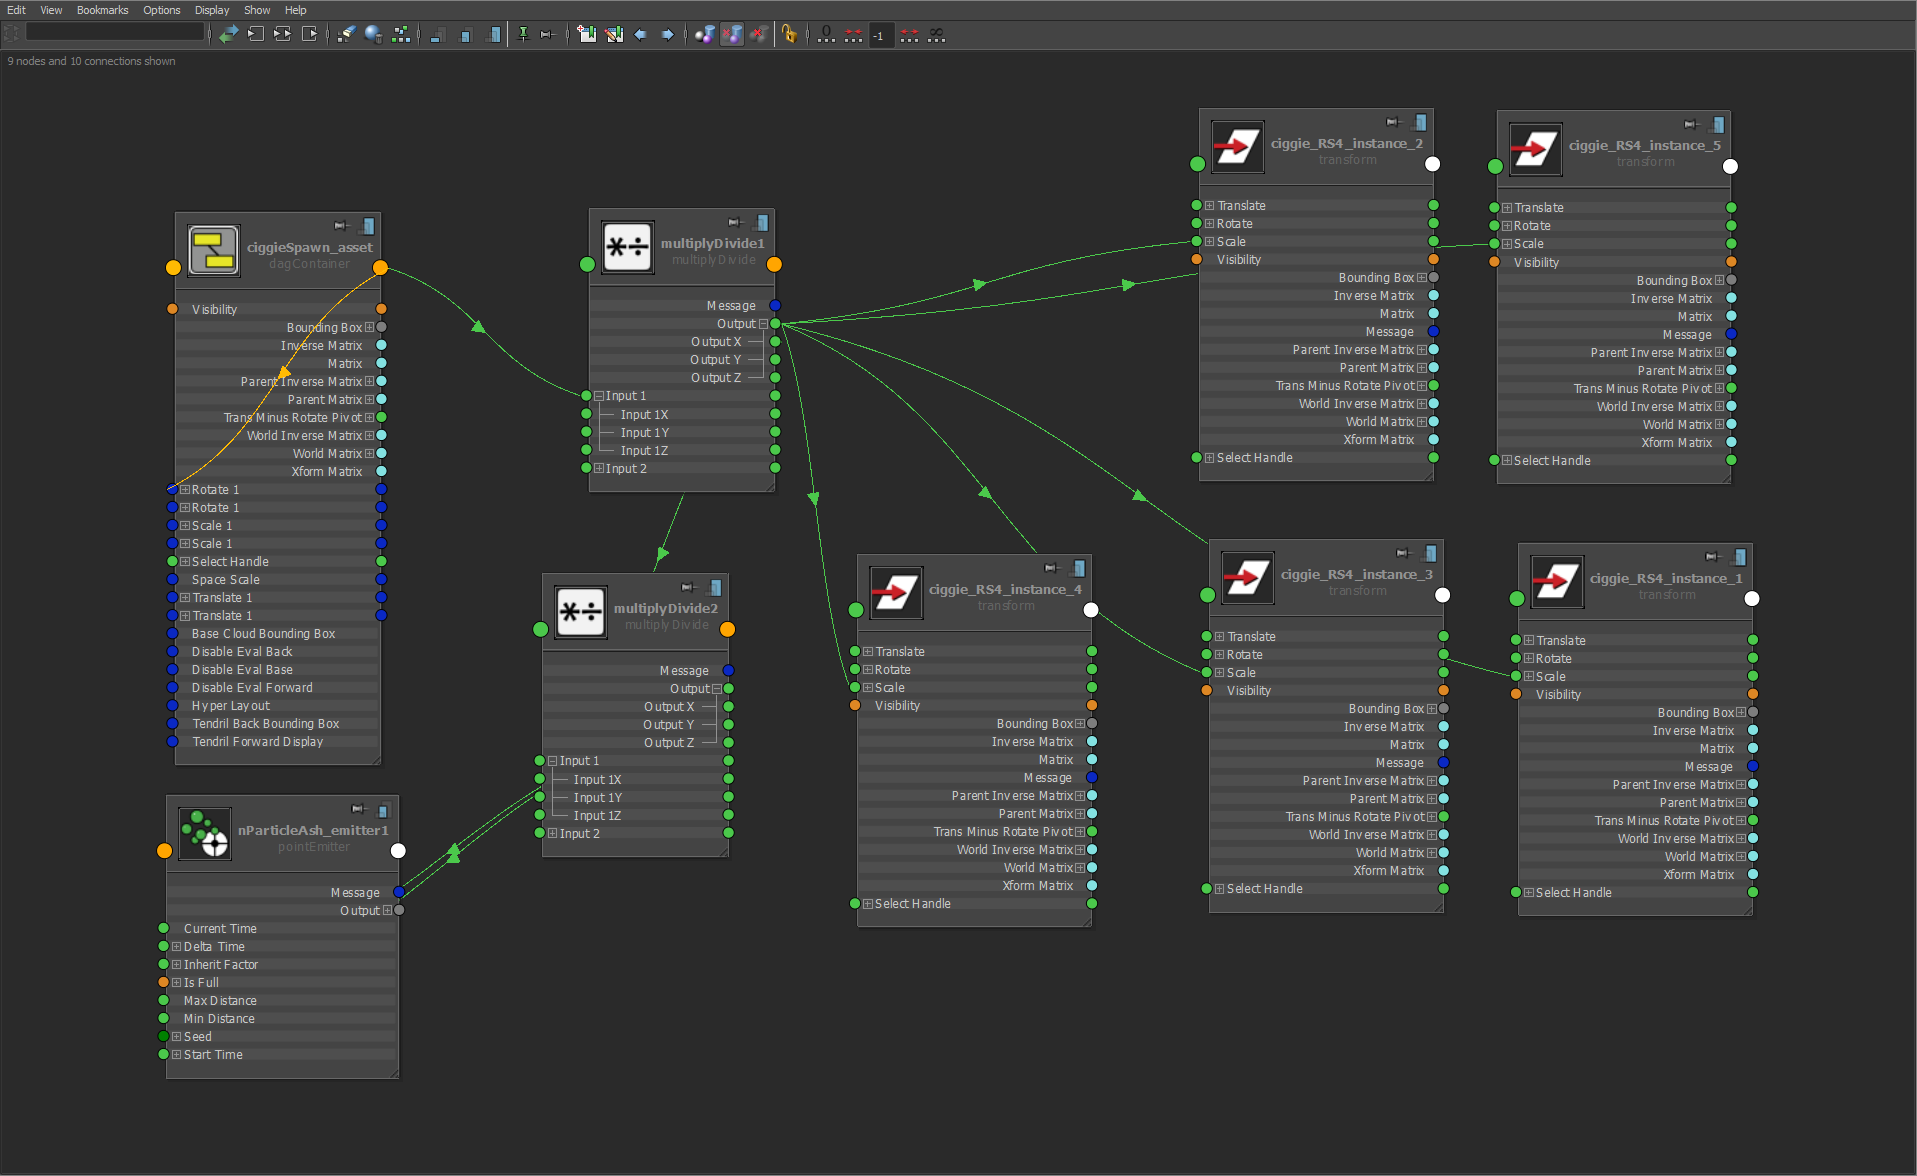
\includegraphics[width=\textwidth]{figures/node-based-editor}
    \caption[Vizuális, csomópont alapú szerkesztő a Maya 3D modellezőben]{Vizuális, csomópont alapú szerkesztő a Maya 3D modellezőben\footnotemark}
    \label{figure:node-based-editor}
\end{figure}
\footnotetext{Forrás: Christian Palmieri: Dynamics and Visual Effects: Studio 2 \\ \url{https://3dpalmieri.wordpress.com/2012/09/13/dynamics-and-visual-effects-studio-2/}}

Sajnos a dolgozat kereteibe nem fért bele egy ilyen eszköz kifejlesztése, ezért egy egyszerűbb megoldást kellett választanom.
A jelenlegi interfész a feladatban található blokkokat egymás alatt jeleníti meg, az összeköttetések pedig név alapján válnak követhetővé.
A szerkesztő az elérhető opciók felsorolásával igyekszik segíteni a felhasználók munkáját.

A feladatok készítésének első lépése, hogy létrehozzuk és elnevezzük az új feladatot.
Ezután a \ref{figure:jporta-exercise}. ábrán látható nézet fogad minket, ahol kialakíthatjuk a feladat belső struktúráját.
Egy lenyitható részben találjuk a hozzáadható blokktípusok listáját.
A feladatban lévő blokkokat dobozok reprezentálják, amelyek bal oldalán sorakoznak a bemeneteik, jobb oldalán a kimeneteik, középen pedig az egyéb tulajdonságaik.
A blokkok összekötését a felhasználni kívánt kimenetek elnevezésével, majd a megfelelő bemeneteknél ezen nevek kiválasztásával tehetjük meg.

\begin{figure}[h]
    \centering
    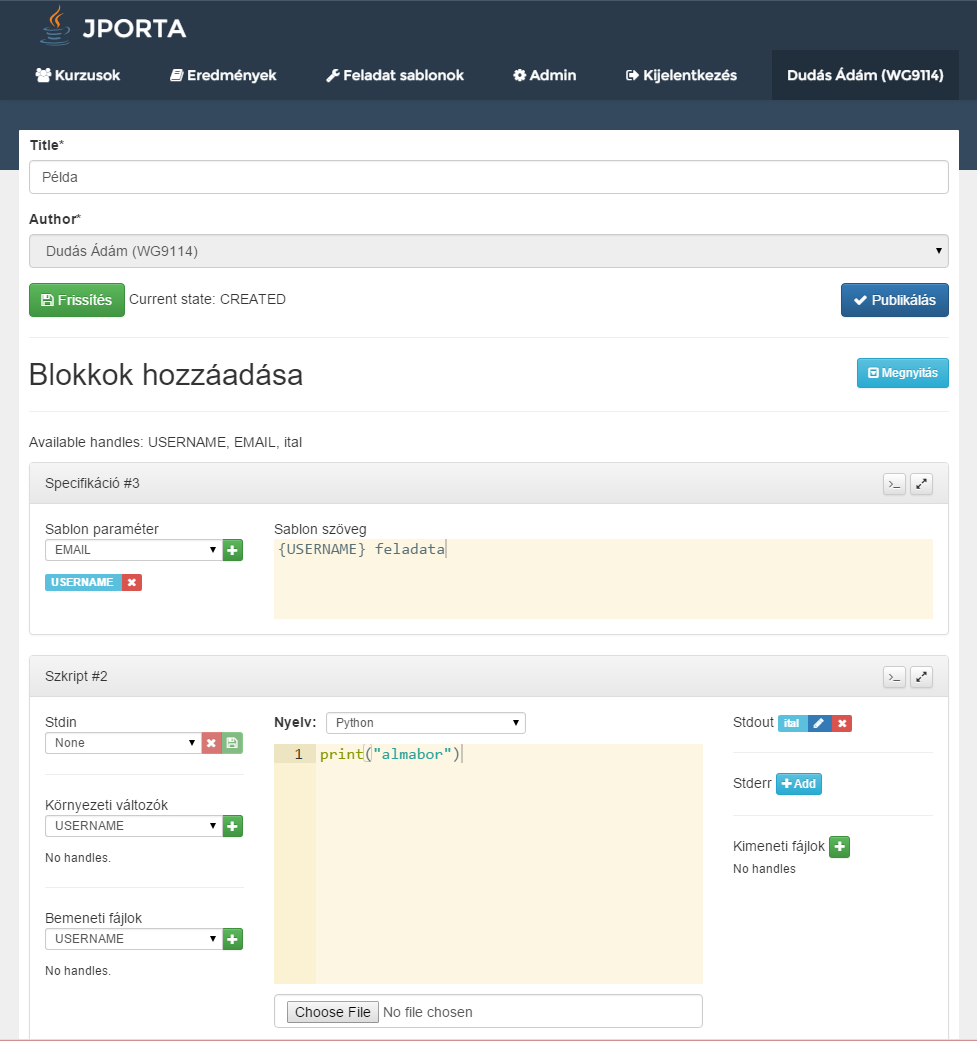
\includegraphics[width=\textwidth]{figures/jporta-exercise}
    \caption{Feladattervező nézet a Jportán}
    \label{figure:jporta-exercise}
\end{figure}

\section{Feladatok kiadása}
Miután a feladatok elkészültek, nincs más hátra, mint kiadni őket a hallgatóknak.
Ehhez két dolgot kell megtennie az oktatónak: egyrészt véglegesíteni kell a feladatot, másrészt hozzá kell rendelni azt a hallgatók egy csoportjához.
Az előbbi a \ref{figure:jporta-exercise}. ábrán is látható \textit{Publikálás} gombbal tehető meg a feladat szerkesztő nézetében.
Erre szintén két okból van szükség.
Egyrészt, ilyenkor végzi el a rendszer a feladat konzisztencia-ellenőrzését: minden kötelező mező kitöltésre került-e, nincs-e a függőségi gráfban kör, stb.
Másrészt, ekkor a feladat véglegesítésre kerül, ezután a lépés után nem lehet további változtatásokat végezni rajta egészen addig, míg visszavonásra nem kerül.
Ez azért nagyon fontos, mert a feladat bármilyen jellegű módosítása érvénytelenné tehetné a feladatra már beérkezett megoldásokat.

Publikálás után a feladat megjelenik a kiadható feladatok listájában, ahhonnan az oktató kiválaszthatja és hozzárendelheti egy kurzushoz vagy kurzuscsoporthoz.
Az összerendeléskor a feladat kiválasztásán túl egy nevet és egy határidőt is meg kell adni.
A feladat és a kiadás különválasztása azért fontos, mert így egy feladatot többször is fel lehet használni, akár különböző kurzusokban vagy szemeszterekben.

\section{Feladatbeadás}\label{section:submission}
A kiadott feladatok megjelennek a rendszerben a hallgatók számára, akik beadásokat készíthetnek ezekre.
Ha a feladat tartalmaz specifikációt, annak kiértékelése a feladatkiadás első megtekintésekor esedékes.
A hallgatók a feladatkiírás alapján elkészítik megoldásaikat, majd a felületen feltöltik a szükséges fájlokat.
Ekkor létrejön a \ref{figure:exercise-uml-cd}. ábrán látható \texttt{Submission} osztály egy egyede, amely összekapcsolja a hallgató által készített állományokat, a feladatkiadást és magát a hallgatót.
A beadás állapota kezdetben \textit{Kiértékelés alatt} (\texttt{under\_evaluation}) lesz.
Ha a feladat tartalmaz kézi beavatkozást igénylő blokkot, ennek ``végrehajtása'' idejére a feladat \textit{Kézi beavatkozásra vár} (\texttt{waiting\_for\_input}) állapotba kerül.
A beadás kiértékelése \textit{Sikeres} (\texttt{successful}) vagy \textit{Sikertelen} (\texttt{failed}) állapotban érhet véget.

A hallgatók a feladatkiadás határidejének lejárta előtt többször is próbálkozhatnak a beadással, akár egy sikeres beadás után is van lehetőségük további javításra.
Beadott megoldásaikat visszamenőleg megtekinthetik a feladatkiadás részletező oldalán.

\section{Megoldások ellenőrzése és értékelése}\label{section:submission-evaluation}
A feladatkiértékelő rendszer második fő feladata a hallgatók által beadott megoldások kiértékelése.
Ahogy az előző szakaszban láthattuk, amikor a hallgató a webportálon beadja a megoldását, létrejön egy \texttt{Submission} típusú objektum, amely ezt a beadást szimbolizálja.
Emellett, a beadás részeként feltöltött fájlokat a rendszer eltárolja, de már nem az eredeti, feltöltéskori nevükkel, hanem annak az azonosítónak a nevével, amelyen az egyes fájlok hivatkozhatóak.
Ha például a feladatban szereplő \texttt{UserFile} blokk \textit{output} nevű kimenetét egy \textit{dokumentáció} elnevezésű azonosítóhoz kapcsoljuk, akkor a fájl neve a fájlrendszerben \textit{dokumentáció} lesz.
Ez azért előnyös, mert így a későbbi fájleléréseknek nem kell egy táblából kiolvasniuk, hogy milyen fájlnév alatt találják meg a keresett erőforrást.
Ugyanakkor bizonyos esetekben szükség lehet a fájl eredeti nevére, például a beadás megtekintésénél zavaró lehetne a hallgató számára, ha az ő általa \textit{első\_specifikációm.docx} néven feltöltött fájlt \textit{dokumentum} fájlnévvel találná meg.
Ilyen jellegű metaadatok tárolására a rendszer a \textit{kiterjesztett fájlattribútumok} (\textit{extended file attributes}) fájlrendszer funkciót használja.
Ez azért praktikus, mert a fájlhoz kötődik, azzal együtt mozog, törlődik, így a konzisztencia megörzésére nem kell további erőforrásokat fordítani.
Ezt a funkciót nagyon sok rendszer támogatja, hátránya viszont, hogy csak limitált mennyiségű adat (körülbelül pár 10 kilobájt) tárolására képes, ami azonban a mi esetünkben bőven elégséges. \cite{wiki:ExtendedFileAttributes}
% xattr: portal fs vs. backup fs támogatja-e

A beadások ezután bekerülnek a kiértékelő modul várakozási sorába aszinkron feldolgozásra, ezzel biztosítva a webportál minél kisebb késleltetését.
Ez a feldolgozási sor a jelenlegi rendszerben Celery segítségével kerül megvalósításra.

A Celery egy Pythonban íródott, nyílt forrású, aszinkron feladatvégrehajtásra specializálódott szoftver, mely elosztott üzenetküldési képességekkel is rendelkezik, ezáltal távoli eljáráshívás implementációjára is alkalmas.
A feladatok végrehajtását a Celery konkurrensen végzi, mégpedig úgy, hogy továbbítja azokat egy vagy több feldolgozófolyamatnak (\textit{worker process}), melyek akár különböző gépeken is elhelyezkedhetnek, teljesítve ezáltal a \ref{section:requirements}. szakaszban említett \ref{req:distributed}. követelményt.
A feldolgozók futhatnak egy, de akár többszálon is, illetve felhasználhatják az eventlet vagy gevent Python-alapú korutin függvénykönyvtárakat is.
A Celery az elosztott üzenetküldés funkciót többféle bróker felhasználásával is meg tudja valósítani, amelyek lehetnek AMQP (pl. RabbitMQ, ZeroMQ), kulcs--érték adatbázis (pl. Redis, MongoDB) vagy relációs adatbázis (SQLAlchemy, Django ORM) alapúak is.
A Jporta esetében a leginkább ajánlott RabbitMQ Advanced Message Queuing Protocol-t megvalósító bróker szoftvert válaszottam az üzenetek szétosztására a végpontok között. \cite{wiki:Celery} \cite{Celery}

% ide lehetne írni a RabbitMQ-ról

A kiértékelő modul ezt a beadásokkal teli várakozási sort dolgozza fel, az egyes feladatok kiértékelését pedig a \ref{section:execution-procedure}. szakaszban leírt módon végzi.
Ilyenkor a folyamat a feladatban található \texttt{SubmissionResult} blokktól indul, ami a feladat eredményét reprezentálja, hiszen ez az, aminek az értékére szükségünk van.
A kiértékelés során minden érintett blokk \texttt{evaluate} metódusa meghívásra kerül, mégpedig egy \texttt{EvaluationContext} típusú paraméterrel.
Ez a ``kiértékelési környezet'' tartamazza a szükséges információkat a kiértékelés végrehajtásához.
A kontextuson keresztül érhetőek el a hallgató által feltöltött fájlok, a hallgató adatai, vagy más külső erőforrás.

Az \texttt{evaluate} metódus törzsében további aszinkron távoli eljáráshívások történhetnek, amelyek szintén Celery révén kerülnek elvégzése, ám ez már nem a feladatkiértékelő modul feladata, hanem a \textit{végrehajtó moduloké}.
A végrehajtó modulok implementálják az olyan fontos feladatokat, mint a forráskódok fordítása, futtatható állományok, szkriptek és tesztek futtatása.
A szükséges végrehajtó modulok a feladatokban felhasznált blokkok implementációjától függenek, magától a kiértékelő modultól, annak működésétől függetlenek, így részletes tárgyalásuk túlmutat a dolgozat keretein.

Az akár helyben, szinkron módon, akár a végrehajtó modulok által máshol, aszinkron módon elvégzett számítások eredményeit -- \textit{produktumait} -- a kiértékelő modul az \texttt{Artifact} osztály felhasználásával tárolja el.
Az \texttt{Artifact} osztály a blokkok kiértékelésének ``melléktermékeit'' szimbolizálja.
Az osztály példányosításához egy azonosítóra és egy kontextusra van szükség, amelyek tartalmazzák a szükséges információt az állományok eléréséhez.
Ahhoz, hogy ezeket a produktumokat egyértelműen azonosítani tudja a rendszer, a következő információkra van szüksége:
\begin{itemize}
    \item a feladat egyedi azonosítója,
    \item a feladatkiadás egyedi azonosítója,
    \item az azonosító neve, amellyel a feladatban a produktumokra hivatkozunk,
    \item ha rendelkezésre áll, a beadás egyedi azonosítója,
    \item ha rendelkezésre áll, a kiértékelést indítványozó felhasználó egyedi azonosítója.
\end{itemize}
Az opcionálisan megjelölt adatok nem minden kiértékelésnél állnak rendelkezésre, például a feladatkiírás kiértékelésénél beadás még nem létezik, így ehhez nem köthető erőforrás.
Ezeken túl az azonosító -- az őt előállító kimenet beállítása révén -- meghatározza a produktum tárolásának módját is.
Vannak olyan produktumok, amelyek perzisztens tárolására nincs szükség, ezért elég, ha a memóriában helyezzük el őket, más produktumokat viszont indokolt lehet fájlokban vagy adatbázisban tárolni.
Az előbbi kategóriába eső produktumokat a Jporta egy Redis tárolóban helyezi el, utóbbiakat rendre a fájlrendszerben vagy a Django által felügyelt relációs adatbázisban.

A Redis egy C nyelven írt, nyílt forráskódú, memóriabeli kulcs--adatszerkezet tároló, amely használható adatbázisként, gyorsítótárként vagy -- az előzőekben már említett -- üzenet brókerként is.
\cite{Redis}  % ide még lehetne írni a Redisről
A Jporta implementációjánál kiváló gyorsítótár tulajdonsága, és átfogó utasításkészlete miatt választottam.

% Fejlesztés menete: git, Vim, CIRCLE devenv

\section{Összegzés}
Ebben a fejezetben ismertettem a Jporta új feladatkiértékelő alrendszerének tervezési lépéseit.
Bemutattam, hogyan képes a rendszer feladatok leírására, illetve miként állíthatóak össze benne új feladatok.
Ezután röviden leírtam a feladatkiadás és -beadás működését, hogy végül eljuthassunk a beadások kiértékelésének problémájához.
Az általam vázolt megoldás ugyan megvalósítja az elvárt funkcionalitást, de a dolgozat írásának idején még közel sem tekinthető késznek.

A funkció csak kezdetlegesen került beágyazásra a Jporta felületébe, továbbá véleményem szerint a \ref{section:exercise-creation}. szakaszban vázolt vizuális szerkesztőeszköz sokat javítana a feladatkészítés folyamatának ergonómiáján.
Hiányos még a rendelkezésre álló blokkok listája is, amelyek sokszor félkész megoldásként szolgálhatnának a feladatok összeállításánál.
Elkészült azonban a blokkok egy csoportja, amelyeket a következő szakasz részletez.

\subsection{Elkészült blokkok}
Ebben a szakaszban sorraveszem és röviden bemutatom az elkészült blokktípusokat.

\subsubsection{AuthorFile}
\textbf{Leírás:} a feladat szerzője által feltöltött fájlt tartalmazó blokk \\
\textbf{Tulajdonságok:} -- \\
\textbf{Bemenetek:} -- \\
\textbf{Kimenetek:}
\begin{itemize}
    \item output: a szerző által feltöltött fájl tartalma
\end{itemize}
        
\subsubsection{Checker}
\textbf{Leírás:} a megoldáson futtatott tesztek eredményét egyszerű sablon-behelyettesítéssel vizsgáló blokk \\
\textbf{Tulajdonságok:}
\begin{itemize}
    \item expected: az elvárt eredmény sablonja, melybe a \texttt{params} bemenet értékeit behelyettesítve kapjuk meg az elvárt eredményt
\end{itemize}
\textbf{Bemenetek:}
\begin{itemize}
    \item actual: a teszt lefutása során kapott eredmény
    \item params: az elvárt eredmény sablonjába behelyettesítendő értékek
\end{itemize}
\textbf{Kimenetek:}
\begin{itemize}
    \item result: az ellenőrzés eredménye
\end{itemize}

\subsubsection{DefaultValue}
\textbf{Leírás:} a végrehajtási kontextusban alapból elérhető értékeket szolgáltató blokk \\
\textbf{Tulajdonságok:} -- \\
\textbf{Bemenetek:} -- \\
\textbf{Kimenetek:}
\begin{itemize}
    \item email: az éppen kiértékelt megoldás szerzőjének e-mail címe
    \item username: az éppen kiértékelt megoldás szerzőjének felhasználóneve
\end{itemize}

\subsubsection{GccCompiler}
\textbf{Leírás:} egy forrásfájl fordítást végző blokk, ami a GCC fordítót használja \\
\textbf{Tulajdonságok:}
\begin{itemize}
    \item extra\_arguments: tetszőleges egyéb parancssori argumentumokat tartalmazó sztring a fordító számára
\end{itemize}
\textbf{Bemenetek:}
\begin{itemize}
    \item files\_in: egyéb bemeneti fájlok, melyeket a fordítási folyamat felhasználhat
    \item libraries: függvénykönytárak
    \item sources: fordítandó forrásfájlok
    \item stdin: szabványos bemenet
\end{itemize}
\textbf{Kimenetek:}
\begin{itemize}
    \item files\_out: egyéb kimeneti fájlok, melyek a fordítás során keletkeztek vagy módosultak
    \item runnable: a fordítás során keletkezett futtatható állomány
    \item stderr: szabványos hibakimenet
    \item stdout: szabványos kimenet
\end{itemize}

\subsubsection{LecturerApproval}
\textbf{Leírás:} valamilyen eredmény oktató által történő kézi értékelését jelző blokk \\
\textbf{Tulajdonságok:} -- \\
\textbf{Bemenetek:}
\begin{itemize}
    \item dependencies: azok az értékek, amelyekre a kézi értékeléshez szükség van
\end{itemize}
\textbf{Kimenetek:}
\begin{itemize}
    \item result: a kézi értékelés eredménye
\end{itemize}

\subsubsection{Runner}
\textbf{Leírás:} futtatható állomány futtatását végző blokk \\
\textbf{Tulajdonságok:} -- \\
\textbf{Bemenetek:}
\begin{itemize}
    \item environment: környezeti változók a futtatás során
    \item files\_in: bemeneti fájlok, melyeket a futtatott állomány felhasználhat
    \item runnable: a futtatandó állomány
    \item stdin: szabványos bemenet
\end{itemize}
\textbf{Kimenetek:}
\begin{itemize}
    \item files\_out: kimeneti fájlok, melyek a futás során keletkeztek vagy módosultak
    \item stderr: szabványos hibakimenet
    \item stdout: szabványos kimenet
\end{itemize}

\subsubsection{Script}
\textbf{Leírás:} a feladat létrehozásakor megadott szkriptet futtató blokk \\
\textbf{Tulajdonságok:}
\begin{itemize}
    \item language: a programnyelv, amelyen a szkript íródott
\end{itemize}
\textbf{Bemenetek:}
\begin{itemize}
    \item environment: környezeti változók a futtatás során
    \item files\_in: bemeneti fájlok, melyeket a futtatott szkript felhasználhat
    \item stdin: szabványos bemenet
\end{itemize}
\textbf{Kimenetek:}
\begin{itemize}
    \item files\_out: kimeneti fájlok, melyek a futás során keletkeztek vagy módosultak
    \item stderr: szabványos hibakimenet
    \item stdout: szabványos kimenet
\end{itemize}

\subsubsection{Specification}
\textbf{Leírás:} feladat specifikációját megadó blokk \\
\textbf{Tulajdonságok:}
\begin{itemize}
    \item template\_text: a specifikáció szövegének sablonja
\end{itemize}
\textbf{Bemenetek:}
\begin{itemize}
    \item template\_params: a specifikáció szövegének sablonjába behelyettesítendő értékek
\end{itemize}
\textbf{Kimenetek:} --

\subsubsection{SubmissionResult}
\textbf{Leírás:} a feladatra adott megoldás eredményét megadó blokk \\
\textbf{Tulajdonságok:} -- \\
\textbf{Bemenetek:}
\begin{itemize}
    \item source: a megoldás eredménye
\end{itemize}
\textbf{Kimenetek:} --

\subsubsection{UserFile}
\textbf{Leírás:} a hallgató által a megoldásához feltöltött fájlt tartalmazó blokk \\
\textbf{Tulajdonságok:}
\begin{itemize}
    \item allowed\_extensions: a feltöltött fájl engedélyezett kiterjesztései
    \item size\_limit: a feltölthető fájl maximális mérete
\end{itemize}
\textbf{Bemenetek:} -- \\
\textbf{Kimenetek:}
\begin{itemize}
    \item output: a hallgató által feltöltött fájl tartalma
\end{itemize}
